\section{Implementation Details} \label{sec:implementation_details}

For our evaluation, we need to determine the road segment for each time point, configure our solver to solve the optimization problem, and provide
the time points $\{t_i\}_{i=1,\dots,n}$.

\subsection{Road Segments}

For our double integrator model, we subdivide the road into segments primarily based on curvature.
As discussed in \ref{subsubsec:limitations_on_qe} and \ref{subsec:approximation_of_model_dynamics}, this approach expands the model's search space
during planning and facilitates the linearization of the dynamics.
The introduced kinematic single track model assumes the curvature to be linear, which is only practical for the road topology if we allow a piecewise
linear curvature and select the current piece.
We can easily add other road topology constraints to be dependent by the current segment, such as the road width.

Our planner operates on a time horizon, divided into discrete time steps $\{t_i\}_{i=1,\dots,n}$.
For each time point, we seek the state and the transition to the next time point, controlled by the input.
The transition is constrained by the dynamics of the model, the state variables, and the control input through coupling constraints.
To make the dynamics and coupling constraints dependent on the road segment, we need to provide the current road segment for each time point.

Given the start and end of each road segment $\{[s_{i-1}, s_{i}]\}_{i=1,\dots,m}$ and the current position $s$ of the vehicle, with a reference velocity
$v(t)$ which can be time-dependent, we can determine the current road segment for each time point by:
\begin{equation}
	i_{s, \{s_{i}\}_{i=0,\dots,m}, v}: \{t_i\}_{i=1,\dots,n} \to \{1,\dots,m\}, t \mapsto i(t) = \min \left\{ j \mid s + \int_{0}^{t} v(\sigma) d\sigma \leq s_j \right\}
\end{equation}

This function can be used to determine the road segment-dependent variables.
We want to make not only the curvature road segment-dependent but also the road width.
The road width consists of the left $\overline{n}(s)$ and right $\underline{n}(s)$ lane width.
The left lane width can be concave, and the right lane width can be convex.
Thus, our implementation of a road segment includes a linear curvature, a concave and convex lane width, and the length of the segment.
This can be extended to include, for example, the upper velocity limits for each segment.

\subsection{Planner}

The convex discrete-time optimization problem will be solved using an external solver, which we refer to as the planner, as it provides the solution
to the motion planning problem.
Our trajectory planner is parameterized by a tuple $(\text{dim}(x), \text{dim}(u), f, \mathcal{C})$, which includes the dimensions of the state
variables, the dimensions of the control inputs, the dynamics equation represented by $f$, and the coupling constraints represented by $\mathcal{C}$.
The time horizon and discretization are given by $\{t_i\}_{i=0,\dots,n}$.

To construct the variables and constraints for our planner, we need to define the state variables, control inputs, and the constraints that describe
the transitions between states.

First, we define the state variables and control inputs for each time step $t_i$:
\begin{equation}
	x(t_i) \in \mathbb{R}^{dim(x)}, u(t_i) \in \mathbb{R}^{dim(u)}
\end{equation}

The system dynamics differ based on the chosen model:

\textbf{Double Integrator Model:} Given the exact discretization of the double integrator
model in \eqref{eq:discrete_time_dynamics_di}, we define the system dynamics constraint as:
\begin{equation}
	x(t_i) = f_{d,di}(x(t_{i-1}), u(t_{i-1}), t_i - t_{i-1})
\end{equation}

\textbf{Bicycle Model:}
Since the dynamics of the kinematic bicycle model include auxiliary variables, we apply forward Euler discretization to the continuous-time dynamics:
\begin{equation}
	x(t_i) = x(t_{i-1}) + \tilde{f}_{kst}(x(t_{i-1}), u(t_{i-1})) \cdot (t_i - t_{i-1})
\end{equation}
where $\tilde{f}_{kst}$ is defined in \eqref{eq:kst_final_dynamics}.

These system dynamics, combined with the coupling constraints and additional constraints, define the full set of variables and constraints used by
the planner.

Given the initial state $x_{initial}$, we model our initial condition with the constraint $x(t_0) = x_{initial}$.
For our evaluation, we did not impose any additional constraints on the final state.
Instead, we modeled the driving behavior through the objective function.

We implemented our optimization problem using Python with the 'cvxpy' library and solved it using the 'MOSEK' solver \cite{diamond2016cvxpy}.

While our planner primarily relies on hard constraints to ensure feasibility and adherence to system dynamics, real-world scenarios often introduce
uncertainties, disturbances, or conflicting objectives that make strict constraint satisfaction impractical.
To address this, we incorporate soft constraints, which allow for controlled constraint relaxation in exchange for a penalty.
By integrating soft constraints into the optimization framework, we can balance feasibility with optimality, enabling more flexible and robust motion
planning.

\subsection{Soft Constraints}

Soft constraints are used in optimization problems where certain constraints can be violated to some extent, but with a penalty.
This is in contrast to hard constraints, which must be strictly satisfied.
Soft constraints are particularly useful in real-world scenarios where it is often impractical to meet all constraints perfectly.

To incorporate soft constraints into a convex optimization problem, we introduce slack variables and a penalty term in the objective function.
The slack variables measure the extent of constraint violation, and the penalty term ensures that violations are minimized.

Consider a constraint of the form \( g(x) \leq 0 \).
To make this constraint soft, we introduce a slack variable \( s \geq 0 \) and modify the constraint to \( g(x) \leq s \).
We then add a penalty term \( \lambda s \) to the objective function, where \( \lambda \) is a positive weight that controls the trade-off between
minimizing the original objective and satisfying the constraint.

The modified optimization problem can be written as:
\begin{align*}
	\min_{x, s} \quad       & f(x) + \lambda s \\
	\text{subject to} \quad & g(x) \leq s      \\
	                        & s \geq 0
\end{align*}

By adjusting the value of \( \lambda \), we can control the degree to which the soft constraint is enforced.
A larger \( \lambda \) places more emphasis on satisfying the constraint, while a smaller \( \lambda \) allows for greater flexibility in violating
the constraint.

\subsection{Replanning Strategy}

In our simulation, we employed a replanning strategy to implement a feedback mechanism.
In addition to the time horizon, we implemented a fixed time interval, shorter than the time horizon, after which the planner recalculates the
trajectory from the current position of the vehicle.
This replanning mechanism allows the planner to adjust to changes in the environment or deviations from the planned path.
We employed a time discretization of equal intervals for the replanning time interval, and the time intervals increase linearly for the remaining
time horizon.

\begin{figure}[h]
	\centering
	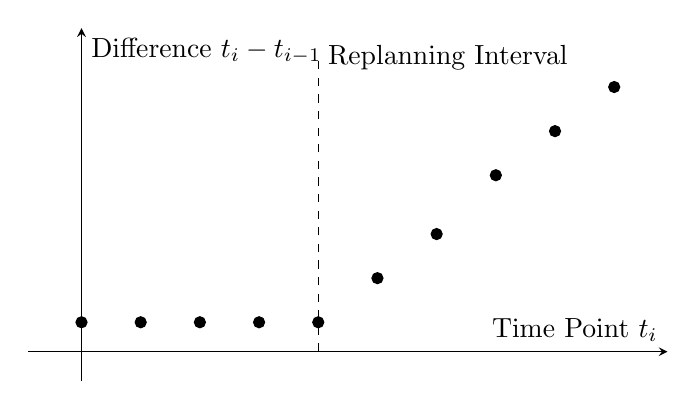
\begin{tikzpicture}
		\begin{axis}[
				xlabel={Time Point $t_i$},
				ylabel={Difference $t_i - t_{i-1}$},
				width=0.8\textwidth,
				height=0.5\textwidth,
				grid=major,
				axis lines=middle,
				enlargelimits=true,
				xtick=\empty, % Remove x-axis ticks
				ytick=\empty, % Remove y-axis ticks
				clip=false
			]
			% Data points
			\addplot[only marks, mark=*, mark size=2pt]
			coordinates {
					(0,0.2) (1,0.2) (2,0.2) (3,0.2) (4,0.2) (5,0.5) (6,0.8) (7,1.2) (8,1.5) (9,1.8)
				};

			% Dashed vertical line for replanning interval
			\addplot[dashed] coordinates {(4,0) (4,2)};

			% Replanning label
			\node[anchor=west] at (axis cs:4,2) {Replanning Interval};

		\end{axis}
	\end{tikzpicture}
	\caption{Time points and their differences to previous time points}
	\label{fig:time_points}
\end{figure}

Figure \ref{fig:time_points} illustrates the time points and their intervals.
The states for the time points to the left of the dashed line are simulated, after which a replanning is triggered.
This replanning follows the same time discretization pattern as the initial planning phase.
The term $\Delta t$ refers to the time intervals between the initial time points, which vary across the different benchmark scenarios.
The slope of time difference after the replanning interval is given by $\Delta^2 t_{replan}$.

Next, we introduce our benchmarking framework, consisting of configurations, such as objectives, road.
